\section{The era of quantum supremacy} \label{sec:era_quant} \index{Quantum supremacy}

\dropcap{A}{} pertinent question to ask is `What is the timescale for useful quantum technologies? When will they be viable?'. The correct answer is likely very soon.

From the perspective of classical computing, Moore's Law (observation!)\index{Moore's Law} for the exponential growth trend in classical computing power has proven to be a very accurate one. In Fig.~\ref{fig:moores_law} we illustrate the historical evolution in classical computing power, and extrapolate 5 years into the future.\index{Moore's Law}

\begin{figure}[!htbp]
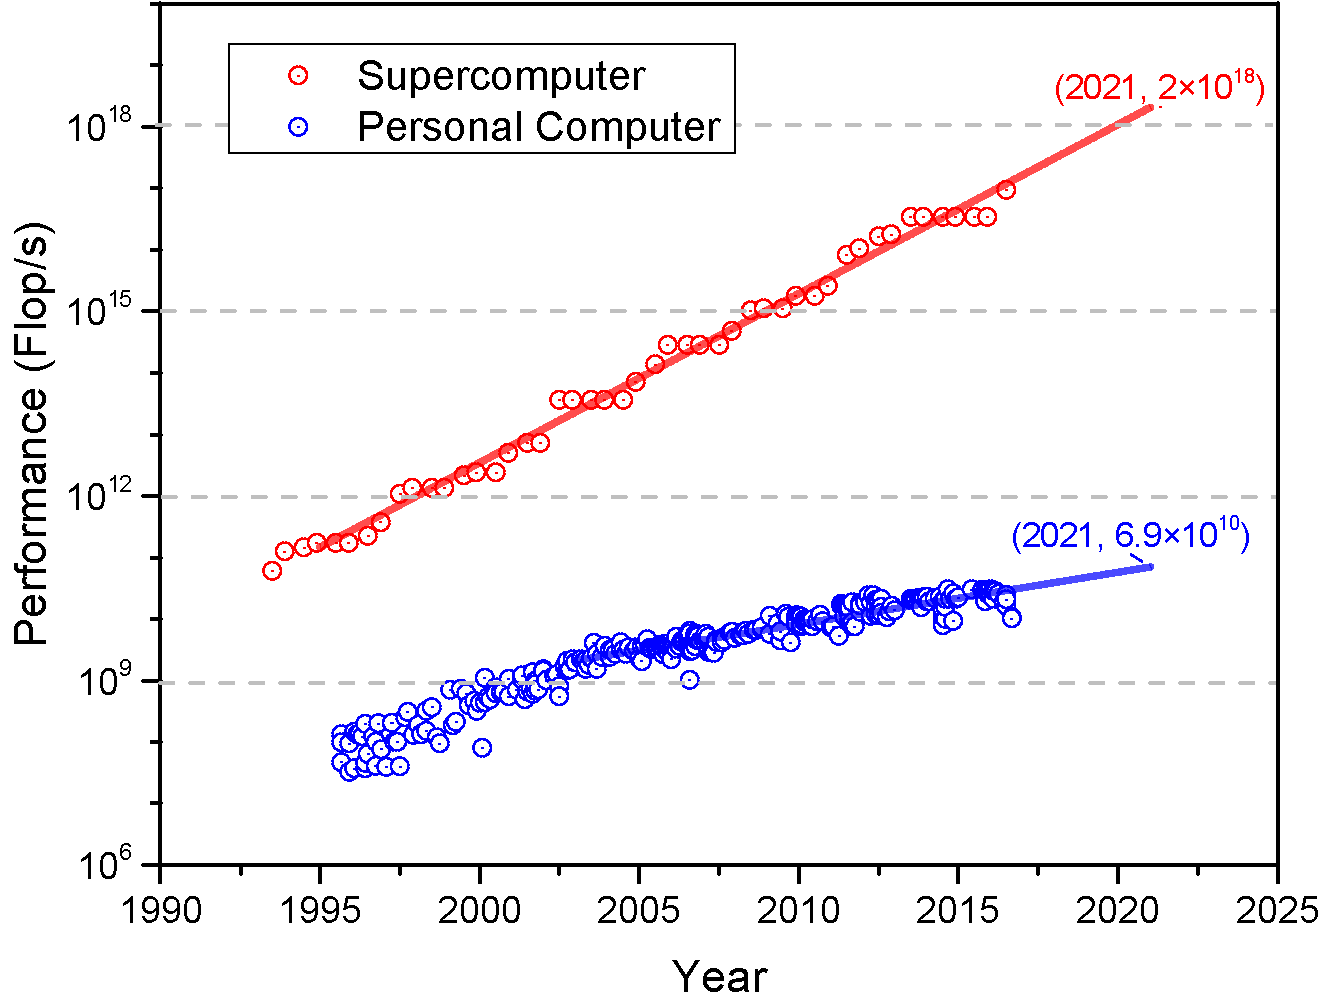
\includegraphics[width=0.475\textwidth]{moores_law}
\captionspacefig \caption{Historical trends in classical computing power for both PCs and top-end supercomputers, with an extrapolation 5 years into the future. The close fit to exponential growth in performance over time is apparent from the logarithmic scale.} \label{fig:moores_law}
\end{figure}

To put this into context, current day microprocessors contains on the order of billions of single transistors. Current day  experimental quantum computers, on the other hand, contain fewer than 100 qubits. We sit at the mere very beginning of Moore's adventure through the quantum era.

%As a comparison we compare this to the \textsc{BosonSampling} \comment{NO BOSON-SAMPLING. MAKE SUPERIMPOSED PLOT COMPRISING ALL ARCHITECTURES AND DEVELOPMENTS. TRY TO EXTRAPOLATE} (Sec.~\ref{sec:BS})\index{Boson-sampling} model for restricted quantum computation, as it is perhaps the most plausible candidate for the first demonstration of quantum computational supremacy. The relationship between \textsc{BosonSampling} photon-number and classical equivalent processing power is shown in Fig.~\ref{fig:moores_super}.

%\begin{figure}[!htbp]
%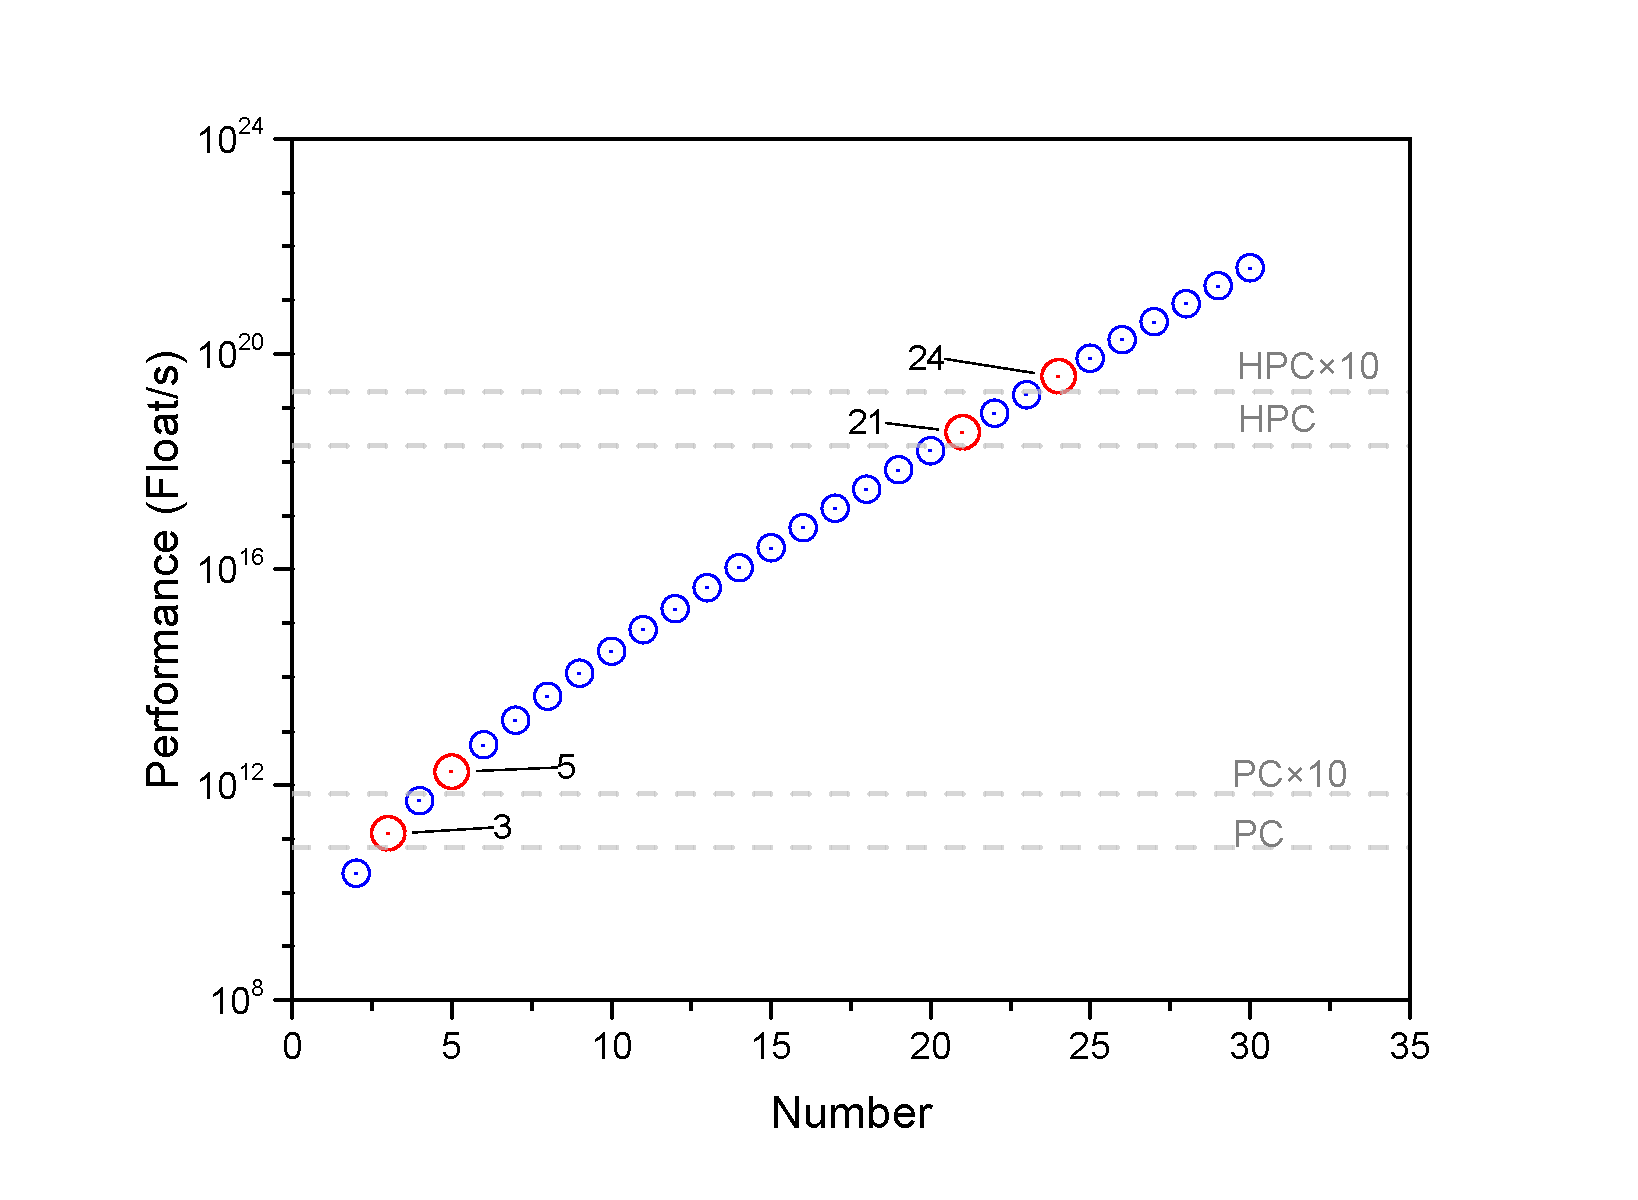
\includegraphics[width=0.475\textwidth]{moores_super}
%\captionspacefig \caption{Relationship between photon-number and classical equivalent FLOPS for `scattershot' \textsc{BosonSampling}. The annotated red data-points show several points of interest, taking a Moore's Law extrapolation of classical computing power 5 years into the future for desktop PCs and top-end high-performance computers, as well as an order of magnitude greater performance respectively. We use these as indicators of the post-classical era.} \label{fig:moores_super}
%\end{figure}

%\comment{Based on these extrapolations}, \cite{CYLu} \comment{(Need to revise the numbers, cite Montanaro et al. on classical simulation of boson-sampling)} \comment{made the prediction that a \textsc{BosonSampling} computer could outperform top-end supercomputers of 5 years into the future by an order of magnitude (a fairly reasonable benchmark for usage of the term `post-classical') using just \mbox{$\sim 24$} photons. Given that present-day experimental efforts have recently reached 10 photons \cite{bib:tenPhotEnt}, with great ambitions to scale up further, it is to be expected that the post-classical era is imminent. Whilst it is difficult to predict exactly when technology will allow a bank of 24 high-fidelity, highly-indistinguishable, push-button (or heralded) single-photon sources operating in parallel, it seems fair to predict that the timescale will be on the order of years rather than decades.}

%\comment{However, be weary that we are being a little optimistic with this statement, since \textsc{BosonSampling} is not universal for quantum computation, and doesn't even have any known practical uses, i.e it's post-classical and that's about it! It would be more helpful to consider prospects for \textit{universal} quantum computation.}

While the power of classical computers scales at most linearly with the number of transistors, the classical-equivalent power\index{Classical-equivalent computational power} of quantum computers scales exponentially with the number of qubits (in the best-case scenario). The classical Moore's Law is close to saturation -- we simply can't make transistors too much smaller than they already are\footnote{Current transistor feature sizes are on the order of several hundred atoms. Under a Moore's Law prediction, we are likely to hit fundamental physical barriers in transistor size within a decade. We can't make a transistor smaller than an atom!}! We therefore envisage a new Quantum Moore's Law, which follows a far more impressive trajectory than its classical counterpart. The point of critical mass in quantum computing will take place when the classical and Quantum Moore's Law extrapolations intersect, signalling the commencement of the \textit{post-classical era}\index{Post-classical era}. Estimating this is more challenging than it sounds, since although the classical Moore's Law is extremely well established with an excellent fit to an exponential trajectory, there aren't yet enough data-points to make a confident prediction about a Quantum Moore's Law, to what trajectory it best fits, and at what rate it progresses.

Aside from quantum computing, theoretically unbreakable quantum crypto-systems, in the form of quantum key distribution (QKD), are already technologically viable\index{Quantum key distribution (QKD)}, and are in fact commercially available off-the-shelf today, as end-to-end units connectable via fibre-optics. Recently, satellite-based QKD was demonstrated, enabling direct intercontinental QKD over thousands of kilometres. Although only a single such satellite has been demonstrated, its success implies that constellations of interconnected such satellites are inevitable in the near future, enabling point-to-point QKD between any two points on Earth. It is likely the next space-race will be the one for quantum supremacy.

As the era of post-classical quantum computation edges closer, the importance of QKD networks will intensify, and along with it the demand for quantum networking infrastructure.

It is clear that humanity already sits at the precipice of harnessing quantum technologies, and must act quickly to enable them to be fully exploited as they emerge in the near future.